% Slides — Capítulo 23 (módulo extra): Mudança Climática
\documentclass[aspectratio=169,11pt]{beamer}
\usepackage{../comum/temameteo}
\graphicspath{{../figuras/cap23/}}

\title[Cap. 23 (extra) --- Mudança Climática]{Capítulo 23 (módulo
extra) --- Mudança Climática}
\subtitle{Meteorologia Prática}
\author{}
\date{}

\begin{document}

\begin{frame}
  \titlepage
  \vfill
  \atribuicao
\end{frame}

\begin{frame}{Roteiro}
  \tableofcontents
\end{frame}

% ---------------------------------------------------------------
\section{A forçante do CO$_2$}

\begin{frame}{O logaritmo das asas}
  \begin{columns}
    \column{0.4\textwidth}
    \eqdestaque{$\Delta F = 5{,}35\,\ln\dfrac{C}{C_0}$;\quad
      $\Delta F_{2\times} = 3{,}7$\,W/m²}
    \vspace{0.4em}
    \begin{itemize}
      \item Centro da banda saturado (Cap.~2); as \alert{asas}
            avançam $\propto\ln C$ (T1; N1).
      \item Hoje ($\sim$420\,ppm): $\Delta F \simeq 2{,}2$\,W/m² —
            visível no espectro de satélite (Cap.~8).
      \item Com feedbacks (Cap.~21): 2,5--4\,K por duplicação; a
            incerteza mora nas nuvens.
    \end{itemize}
    \column{0.6\textwidth}
    \begin{center}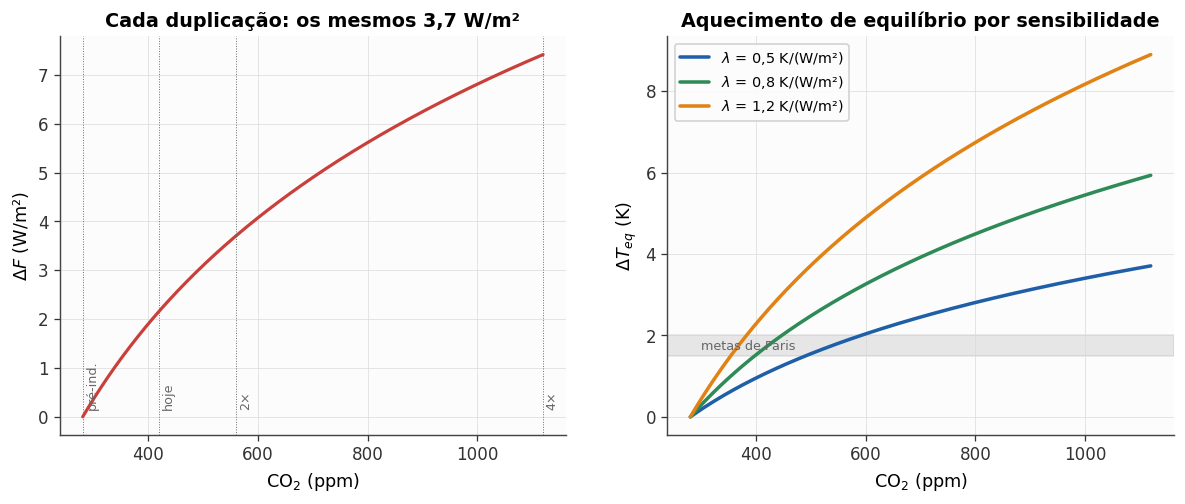
\includegraphics[width=\linewidth]{notebook_forcante.png}\\[-2pt]
    {\tiny forçante e aquecimento por sensibilidade — Caso~1 do notebook do curso}\end{center}
  \end{columns}
\end{frame}

% ---------------------------------------------------------------
\section{A inércia oceânica}

\begin{frame}{Duas caixas: a dívida térmica}
  \begin{columns}
    \column{0.4\textwidth}
    \eqdestaque{$\tau_{rápido} \sim 4$\,anos;\quad
      $\tau_{lento} \sim$ séculos}
    \vspace{0.4em}
    \begin{itemize}
      \item Camada de mistura responde em anos (Pinatubo!); o oceano
            profundo cobra por séculos (T2).
      \item CO$_2$ congelado hoje: ainda $+0{,}4$--0,6\,K de
            aquecimento \alert{comprometido} (Caso~2; N2).
      \item A capacidade térmica da água (Cap.~3) governando o
            século.
    \end{itemize}
    \column{0.6\textwidth}
    \begin{center}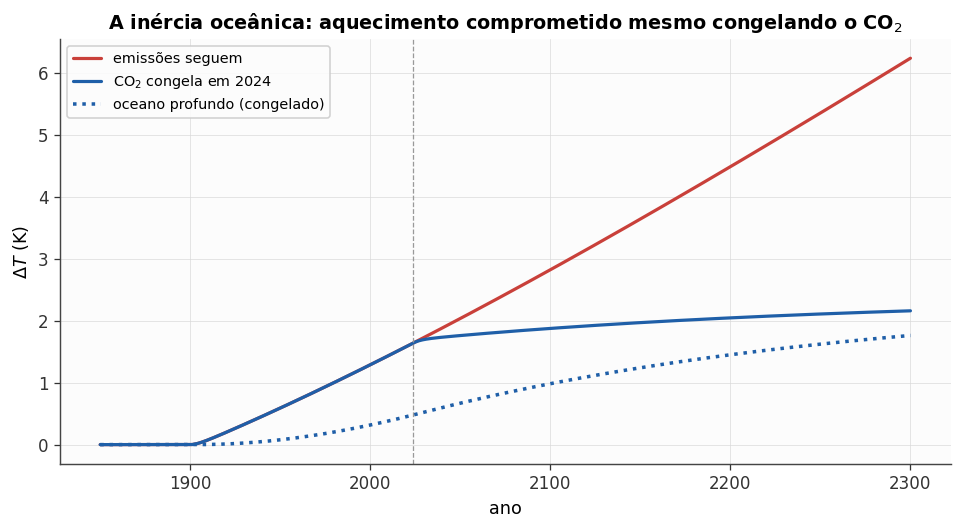
\includegraphics[width=\linewidth]{notebook_duascaixas.png}\\[-2pt]
    {\tiny cenários com o modelo de duas caixas — Caso~2 do notebook do curso}\end{center}
  \end{columns}
\end{frame}

% ---------------------------------------------------------------
\section{O orçamento de carbono}

\begin{frame}{TCRE: cada tonelada conta, e a conta é linear}
  \begin{columns}
    \column{0.4\textwidth}
    \eqdestaque{$\Delta T \simeq 0{,}45$\,K por 1000\,GtCO$_2$}
    \vspace{0.4em}
    \begin{itemize}
      \item Log da forçante × saturação dos sumidouros: os dois se
            cancelam (T4).
      \item Emitidos: $\sim$2500\,GtCO$_2$ ($\to$ 1,2\,K, confere);
            restam
            $\sim$800 para 1,5\,°C ($\approx$ 20 anos no ritmo).
      \item Consequência dura: estabilizar $T$ $=$ emissão líquida
            \alert{zero} (Caso~3; N3).
    \end{itemize}
    \column{0.6\textwidth}
    \begin{center}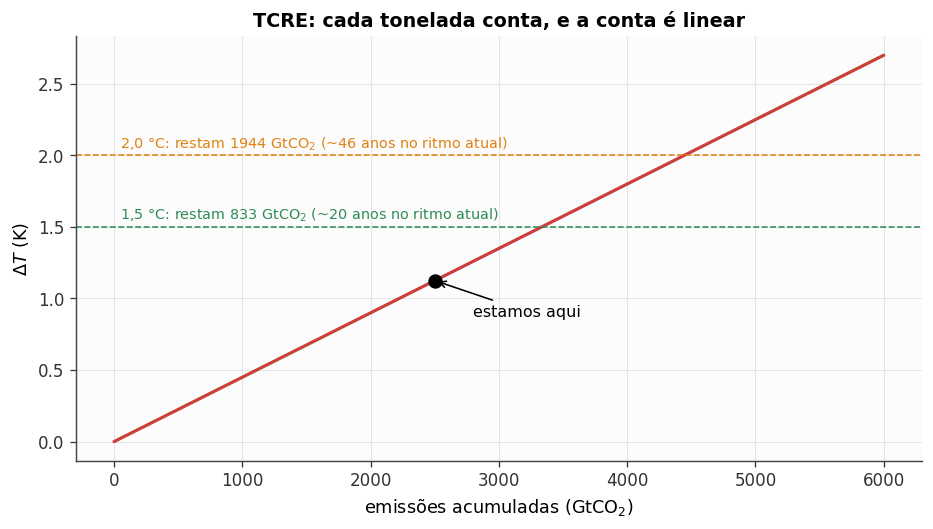
\includegraphics[width=\linewidth]{notebook_tcre.png}\\[-2pt]
    {\tiny o orçamento de carbono — Caso~3 do notebook do curso}\end{center}
  \end{columns}
\end{frame}

% ---------------------------------------------------------------
\section{Detecção e assinaturas}

\begin{frame}{O sinal emergindo do ruído}
  \begin{columns}
    \column{0.4\textwidth}
    \begin{itemize}
      \item ENSO e vulcões (Cap.~21) escondem a tendência por
            décadas: $\sim$30--40 anos para 95\% de detecção
            (Caso~4; N4).
      \item Uma década fria isolada não refuta nada — o teste é
            multidecadal.
      \item Impressão digital (T5): troposfera aquece E estratosfera
            ESFRIA — o Sol aqueceria as duas.
    \end{itemize}
    \column{0.6\textwidth}
    \begin{center}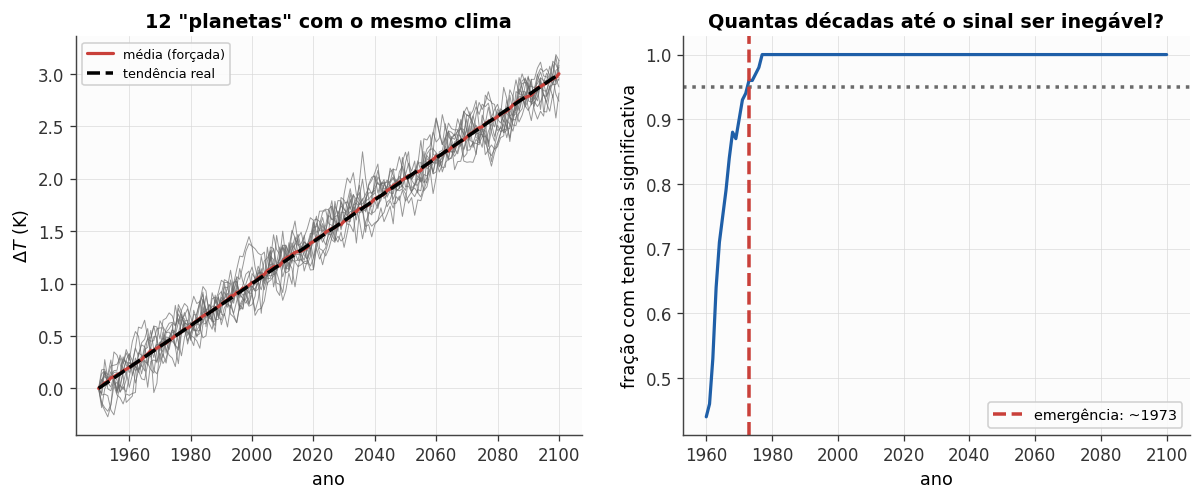
\includegraphics[width=\linewidth]{notebook_deteccao.png}\\[-2pt]
    {\tiny doze ``planetas'' e a emergência do sinal — Caso~4 do notebook do curso}\end{center}
  \end{columns}
\end{frame}

\begin{frame}{Impactos capítulo a capítulo}
  \begin{itemize}
    \item Extremos de chuva: $+7\%$/K de Clausius--Clapeyron
          (Cap.~4).
    \item Ciclones tropicais: teto MPI sobe poucos \%/K, chuva e
          nível do mar compõem (Cap.~16, N3).
    \item Ondas de calor úmido: $T_w$ rumo ao limite fisiológico
          (Cap.~4).
    \item Bloqueios e jato (Cap.~11); nível do mar: expansão térmica
          (T3) $+$ gelo.
    \item Previsão sazonal-decadal como fronteira (Cap.~20).
  \end{itemize}
\end{frame}

% ---------------------------------------------------------------
\section{Síntese e laboratório}

\begin{frame}{O fecho do curso}
  \eqdestaque{$\Delta F = 5{,}35\ln\tfrac{C}{C_0}$ \quad
    $\Delta T = \tfrac{\lambda_0\Delta F}{1-f}$ \quad
    $\tau$: anos e séculos \quad
    $\Delta T = \mathrm{TCRE}\times E_{cum}$}
  \vspace{0.6em}
  Nada de novo entrou: estufa (Cap.~2), feedbacks (Cap.~21), oceano
  (Cap.~3) e estatística × caos (Cap.~20) — o mesmo curso que prevê a
  chuva de amanhã fecha o balanço do século.
\end{frame}

\begin{frame}{Laboratório numérico --- notebook do Cap.~23}
  \texttt{notebooks/cap23\_mudanca.ipynb}
  \begin{enumerate}
    \item Forçante log e cenários por sensibilidade.
    \item Duas caixas: o aquecimento comprometido.
    \item TCRE e o orçamento de carbono.
    \item Emergência do sinal no ruído.
  \end{enumerate}
  \vspace{0.4em}
  \textbf{Exercícios}: T1--T5 e N1--N4 nas notas; células reservadas no
  notebook.
  \vfill
  \atribuicao
\end{frame}

\end{document}
